\documentclass[12pt]{article}
%%---------------------------------------------------------------------
% packages
% geometry
\usepackage{geometry}
% font
\usepackage{fontspec}
\defaultfontfeatures{Mapping=tex-text}  %%如果没有它,会有一些 tex 特殊字符无法正常使用,比如连字符。
\usepackage{xunicode,xltxtra}
\usepackage[BoldFont,SlantFont,CJKnumber,CJKchecksingle]{xeCJK}  % \CJKnumber{12345}: 一万二千三百四十五
\usepackage{CJKfntef}  %%实现对汉字加点、下划线等。
\usepackage{pifont}  % \ding{}
% math
\usepackage{amsmath,amsfonts,amssymb}
% color
\usepackage{color}
\usepackage{xcolor}
\definecolor{EYE}{RGB}{199,237,204}
\definecolor{FLY}{RGB}{128,0,128}
\definecolor{ZHY}{RGB}{139,0,255}
% graphics
\usepackage[americaninductors,europeanresistors]{circuitikz}
\usepackage{tikz}
\usetikzlibrary{positioning,arrows,shadows,shapes,calc,mindmap,trees,backgrounds}  % placements=positioning
\usepackage{graphicx}  % \includegraphics[]{}
\usepackage{subfigure}  %%图形或表格并排排列
% table
\usepackage{colortbl,dcolumn}  %% 彩色表格
\usepackage{multirow}
\usepackage{multicol}
\usepackage{booktabs}
% code
\usepackage{fancyvrb}
\usepackage{listings}
% title
\usepackage{titlesec}
% head/foot
\usepackage{fancyhdr}
% ref
\usepackage{hyperref}
% pagecolor
\usepackage[pagecolor={EYE}]{pagecolor}
% tightly-packed lists
\usepackage{mdwlist}

\usepackage{styles/iplouccfg}
\usepackage{styles/zhfontcfg}
\usepackage{styles/iplouclistings}

%%---------------------------------------------------------------------
% settings
% geometry
\geometry{left=2cm,right=1cm,top=2cm,bottom=2cm}  %设置 上、左、下、右 页边距
\linespread{1.5} %行间距
% font
\setCJKmainfont{Adobe Kaiti Std}
%\setmainfont[BoldFont=Adobe Garamond Pro Bold]{Apple Garamond}  % 英文字体
%\setmainfont[BoldFont=Adobe Garamond Pro Bold,SmallCapsFont=Apple Garamond,SmallCapsFeatures={Scale=0.7}]{Apple Garamond}  %%苹果字体没有SmallCaps
\setCJKmonofont{Adobe Fangsong Std}
% graphics
\graphicspath{{figures/}}
\tikzset{
    % Define standard arrow tip
    >=stealth',
    % Define style for boxes
    punkt/.style={
           rectangle,
           rounded corners,
           draw=black, very thick,
           text width=6.5em,
           minimum height=2em,
           text centered},
    % Define arrow style
    pil/.style={
           ->,
           thick,
           shorten <=2pt,
           shorten >=2pt,},
    % Define style for FlyZhyBall
    FlyZhyBall/.style={
      circle,
      minimum size=6mm,
      inner sep=0.5pt,
      ball color=red!50!blue,
      text=white,},
    % Define style for FlyZhyRectangle
    FlyZhyRectangle/.style={
      rectangle,
      rounded corners,
      minimum size=6mm,
      ball color=red!50!blue,
      text=white,},
    % Define style for zhyfly
    zhyfly/.style={
      rectangle,
      rounded corners,
      minimum size=6mm,
      ball color=red!25!blue,
      text=white,},
    % Define style for new rectangle
    nrectangle/.style={
      rectangle,
      draw=#1!50,
      fill=#1!20,
      minimum size=5mm,
      inner sep=0.1pt,}
}
\ctikzset{
  bipoles/length=.8cm
}
% code
\lstnewenvironment{VHDLcode}[1][]{%
  \lstset{
    basicstyle=\footnotesize\ttfamily\color{black},%
    columns=flexible,%
    framexleftmargin=.7mm,frame=shadowbox,%
    rulesepcolor=\color{blue},%
%    frame=single,%
    backgroundcolor=\color{yellow!20},%
    xleftmargin=1.2\fboxsep,%
    xrightmargin=.7\fboxsep,%
    numbers=left,numberstyle=\tiny\color{blue},%
    numberblanklines=false,numbersep=7pt,%
    language=VHDL%
    }\lstset{#1}}{}
\lstnewenvironment{VHDLmiddle}[1][]{%
  \lstset{
    basicstyle=\scriptsize\ttfamily\color{black},%
    columns=flexible,%
    framexleftmargin=.7mm,frame=shadowbox,%
    rulesepcolor=\color{blue},%
%    frame=single,%
    backgroundcolor=\color{yellow!20},%
    xleftmargin=1.2\fboxsep,%
    xrightmargin=.7\fboxsep,%
    numbers=left,numberstyle=\tiny\color{blue},%
    numberblanklines=false,numbersep=7pt,%
    language=VHDL%
    }\lstset{#1}}{}
\lstnewenvironment{VHDLsmall}[1][]{%
  \lstset{
    basicstyle=\tiny\ttfamily\color{black},%
    columns=flexible,%
    framexleftmargin=.7mm,frame=shadowbox,%
    rulesepcolor=\color{blue},%
%    frame=single,%
    backgroundcolor=\color{yellow!20},%
    xleftmargin=1.2\fboxsep,%
    xrightmargin=.7\fboxsep,%
    numbers=left,numberstyle=\tiny\color{blue},%
    numberblanklines=false,numbersep=7pt,%
    language=VHDL%
    }\lstset{#1}}{}
% pdf
\hypersetup{%pdfpagemode=FullScreen,%
            pdfauthor={Haiyong Zheng},%
            pdftitle={Title},%
            CJKbookmarks=true,%
            bookmarksnumbered=true,%
            bookmarksopen=false,%
            plainpages=false,%
            colorlinks=true,%
            citecolor=green,%
            filecolor=magenta,%
            linkcolor=cyan,%red(default)
            urlcolor=cyan}
% section
%http://tex.stackexchange.com/questions/34288/how-to-place-a-shaded-box-around-a-section-label-and-name
\newcommand\titlebar{%
\tikz[baseline,trim left=3.1cm,trim right=3cm] {
    \fill [cyan!25] (2.5cm,-1ex) rectangle (\textwidth+3.1cm,2.5ex);
    \node [
        fill=cyan!60!white,
        anchor= base east,
        rounded rectangle,
        minimum height=3.5ex] at (3cm,0) {
        \textbf{\thesection.}
    };
}%
}
\titleformat{\section}{\Large\bf\color{blue}}{\titlebar}{0.1cm}{}
% head/foot
\setlength{\headheight}{15pt}
\pagestyle{fancy}
\fancyhf{}

\chead{\color{black!50!green}Assignment \#3}

%\lfoot{\color{blue!50!green}Dai Jialun}
\cfoot{\color{blue!50!green}\href{http://vision.ouc.edu.cn/~zhenghaiyong}{CVBIOUC}}
\rfoot{\color{blue!50!green}$\cdot$\ \thepage\ $\cdot$}
\renewcommand{\headrulewidth}{0.4pt}
\renewcommand{\footrulewidth}{0.4pt}

%%---------------------------------------------------------------------
\begin{document}
%%---------------------------------------------------------------------
%%---------------------------------------------------------------------
% \titlepage
\title{\vspace{-2em}CV2015Spring---Assignment \#\textbf{3}\\
\normalsize{Due: June 18, 2015 (12:00AM)}}
\author{Dai Jialun, Wang Ruchen}
%\date{\vspace{-0.7em}May 30, 2015\vspace{-0.7em}}
%%---------------------------------------------------------------------
\maketitle\thispagestyle{fancy}
%%---------------------------------------------------------------------
\maketitle
%\tableofcontents 


%\section{Programming problem: salient object detection}
\section{Assignment requirement}

For this assignment, you will implement segmentation through grab cut and meanshift. Then, evaluate each method by adjusting parameters in segmentation. See Figure~\ref{fig: result1} and Figure~\ref{fig: result2} for examples.
\begin{figure}[!ht]
  \centering 
  \subfigure[Input image]{ 
    \label{fig: result: a} %% label for first subfigure 
    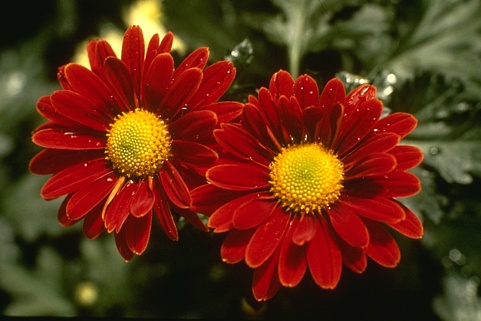
\includegraphics[width=0.31\textwidth]{origin}} 
  \subfigure[Segmentation result]{ 
    \label{fig: result: b} %% label for second subfigure 
    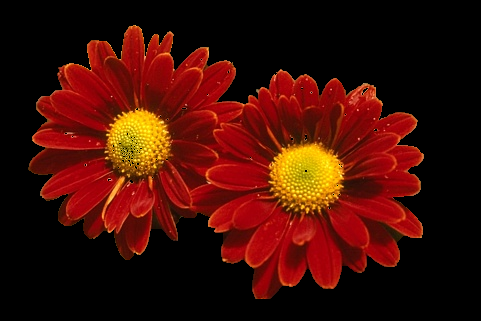
\includegraphics[width=0.31\textwidth]{segmentation}} 
  \subfigure[Evaluation]{ 
    \label{fig: result: c} %% label for second subfigure 
    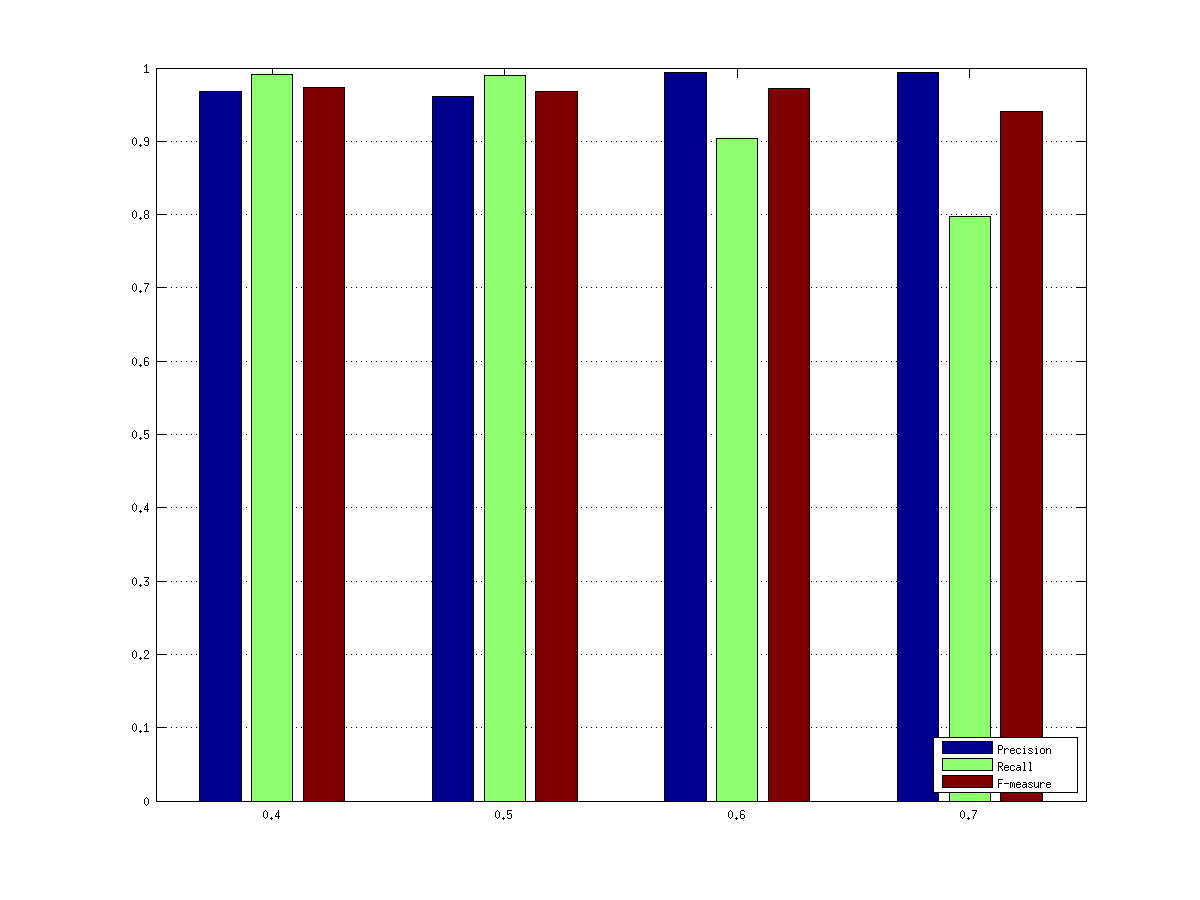
\includegraphics[width=0.28\textwidth]{evaluation}} 
  \caption{Grab cut}
  \label{fig: result1} %% label for entire figure 
\end{figure}

\begin{figure}[!ht]
\centering
 % \caption{Salient object detection.}
%  \label{fig: result} %% label for entire figure 
  \subfigure[Input image]{ 
    \label{fig: result: d} %% label for first subfigure 
    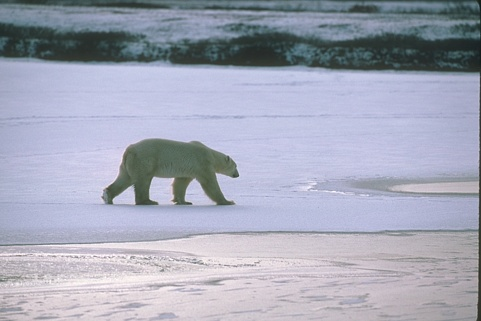
\includegraphics[width=0.31\textwidth]{100007}} 
  \subfigure[Segmentation result]{ 
    \label{fig: result: e} %% label for second subfigure 
    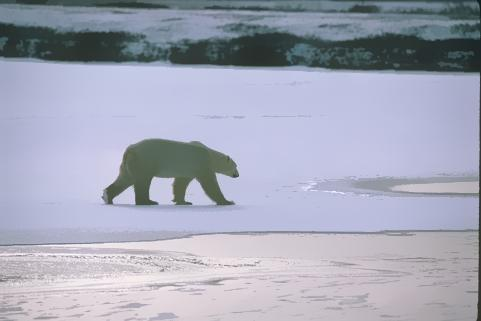
\includegraphics[width=0.31\textwidth]{100007MS}} 
  \subfigure[Evaluation]{ 
    \label{fig: result: f} %% label for second subfigure 
    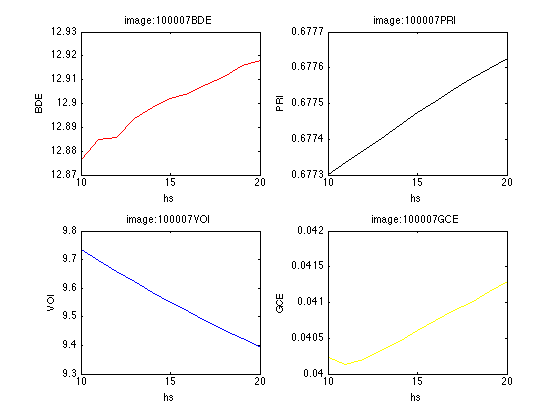
\includegraphics[width=0.28\textwidth]{eval.png}} 
  \caption{Mean shift}
  \label{fig: result2} %% label for entire figure 
\end{figure}

%Your method must be region-based, and at least one feature and one prior should be used. I will give you some tips for the implementation in the following sections.

\section{Grab Cut (60 points)}

The whole framework of the implementation for evaluation of grab cut is shown in Figure~\ref{fig: framework}, it may serve as a reference for your assignment.
In this part, what you need to do:
\begin{enumerate}
\item Implement image signature, grab cut and evaluation (20 points).
\item Adjust one parameter (see~\ref{note}) to obtain different segmentation results, then evaluate (20 points).
\item Adjust another parameter (see~\ref{note}) to obtain different segmentation results and evaluate (20 points).
\end{enumerate}
Next, I will introduce the implementation and requirement of each part of the framework.


\begin{figure}[!ht]
\centering
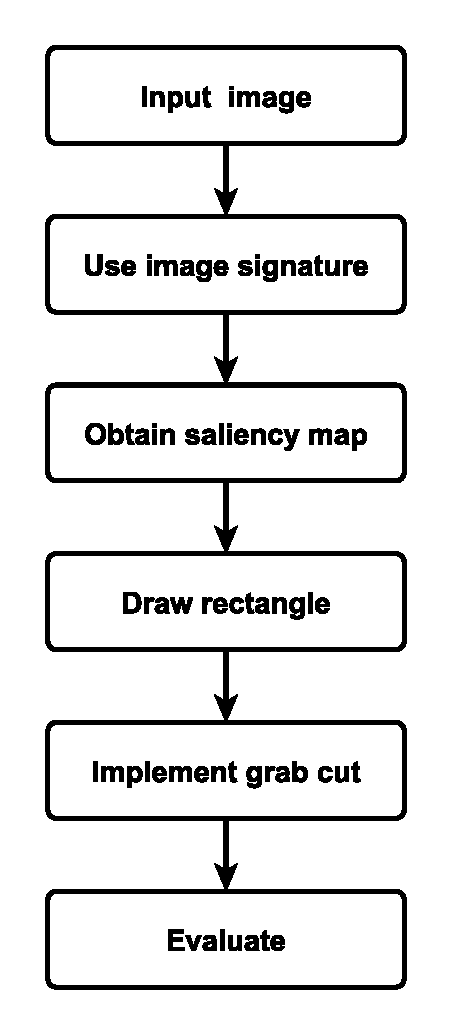
\includegraphics[width=0.2\textwidth]{SIG_GRAB.eps}
\caption{Framework of the implementation for evaluation of grab cut.}
\label{fig: framework}
\end{figure}

\subsection{Step 1: Input image}

A simple dataset (PASCAL) can be downloaded from the website\footnote{\url{http://vision.ouc.edu.cn/~zhenghaiyong/courses/cv/2015spring/assignments/PASCAL.zip}}. The dataset contains input images and groundtruth. Use all images (850 images totally) from the dataset for segmentation, and evaluate grab cut by adjusting different parameters. 

Here, I just pick one image for segmentation and evaluation as an example and the parameter I choose to adjust is {\color{blue} threshold} in step 3.

\subsection{Step 2: Use image signature}

\begin{description}
\item[Input] The input color image ($m \times n \times 3$ matrix).
\item[Output] The saliency map ($m \times n$ matrix).
%\item[Implementation] The method of image signature can be used to get the saliency map from input color image. 
\item[Hint] The saliency map is obtained by image signature and the matlab  code of ``signatureSal'' can be downloaded from website\footnote{\url{http://www.vision.caltech.edu/~harel/share/gbvs.php}}, where the files of SIG\_single, signatureSal and default\_signature\_param are used.
\end{description}
%\begin{itemize}
%\item Color information
%\begin{itemize}
%\item[-] You should quantize each color channel (RGB) to reduce the number of colors (such as from $256$ to $16$), then the number of color is reduced to $16 \times 16 \times 16 = 4096$. In order to create a bin for each color, you can use a number ($1 \sim 4096$) instead of (R, G, B) values to represent a color uniquely.
%\end{itemize}
%\item Texture information
%\begin{itemize}
%\item[-] You should compute the LBP value of each pixel here.  
%\end{itemize}
%\end{itemize}
%\item[Hint] The extraction of color/texture information can refer to the matlab code from the website\footnote{\url{http://jianghz.com/projects/saliency_drfi/index.html}}, which also contains the computation of color histogram and texture histogram of superpixels in step 2 and the conversion of superpixel saliency to pixel saliency in step 4.

\begin{figure}[!ht]
  \centering 
  \subfigure[Input image]{ 
    \label{fig: } %% label for first subfigure 
    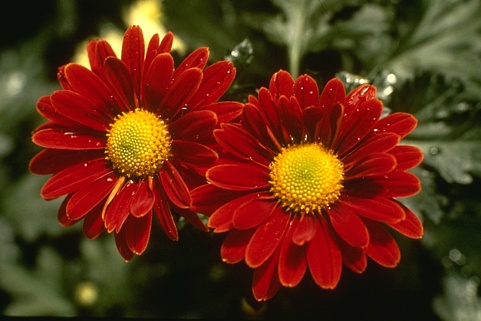
\includegraphics[width=0.3\textwidth]{origin}} 
  \subfigure[Saliency map]{ 
    \label{fig: result1: b} %% label for second subfigure 
    
\includegraphics[width=0.3\textwidth]{saliency}} 
  \caption{Image signature}
  \label{fig: } %% label for entire figure 
\end{figure}


\subsection{Step 3: Draw the rectangle}

\begin{description} 
\item[Input] The input saliency map image ($m \times n$ matrix). 
\item[Output]  A rectangle that is used to initialize the grab cut. %Superpixel segmentation matrix ($m \times n$ matrix), the value of the pixel in this matrix is just a label to indicate the superpixel it belongs to, and pixels of the same superpixel are labeled the same value. 
\item[Hint] 
\begin{itemize}
\item The rectangle is used to locate the most probable position of object and initialize mask in grab cut. 
\item You can use {\color{blue} thresholding} to transform saliency map to binary image and draw a rectangle according to the binary image. The {\color{blue} size of rectangle} is also adjustable.
\end{itemize}
\end{description}

\begin{figure}[!ht]
  \center{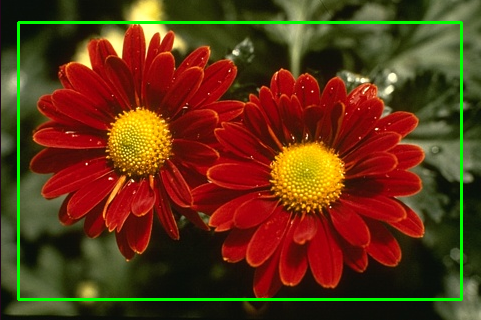
\includegraphics[width=0.3\textwidth]{rectangle}} 
  \caption{Rectangle in input image}
  \label{fig: } %% label for entire figure 
\end{figure}


\begin{comment}
\subsection{Step 3: Get binary image}

\begin{description} 
\item[Input] The input saliency map image ($m \times n$ matrix). 
\item[Output]  The binary image ($m \times n \times 3$ matrix). %Superpixel segmentation matrix ($m \times n$ matrix), the value of the pixel in this matrix is just a label to indicate the superpixel it belongs to, and pixels of the same superpixel are labeled the same value. 
\item[Implement] Set a {\color{blue} threshold} to transform saliency map to binary image to locate the most probable object.
\end{description}

\begin{figure}[!ht]
  \center{
\includegraphics[width=0.3\textwidth]{binary}} 
  \caption{The binary image of saliency map}
  \label{fig: } %% label for entire figure 
\end{figure}


\subsection{Step 4: Draw the rectangle}

\begin{description} 
\item[Input] The binary image ($m \times n$ matrix). 
\item[Output]  A rectangle that is used to initialize the grab cut.%Superpixel segmentation matrix ($m \times n$ matrix), the value of the pixel in this matrix is just a label to indicate the superpixel it belongs to, and pixels of the same superpixel are labeled the same value. 
\item[Hint] A rectangle that contains all white pixel in the binary image is used to initialize mask in grab cut. You can adjust {\color{blue} size of the rectangle} to get different results.
\end{description}

\begin{figure}[!ht]
  \center{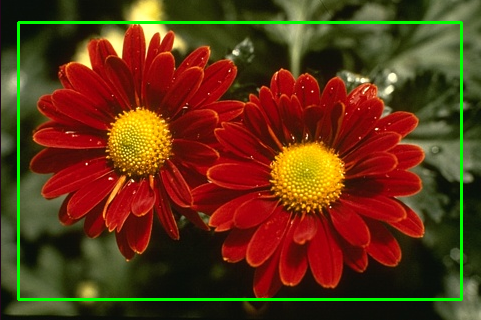
\includegraphics[width=0.3\textwidth]{rectangle}} 
  \caption{Rectangle in input image}
  \label{fig: } %% label for entire figure 
\end{figure}
\end{comment}




\subsection{Step 4: Implement grab cut}

\begin{description}
\item[Input] The input image ($m \times n \times 3$ matrix) from step 1, and the rectangle that you computed from step 3.
\item[Output] The image after segmentation ($m \times n \times 3$ matrix).
\item[Implementation] Use grab cut with the rectangle to initialize and iterate $k$ {\color{blue} times} for segmentation.
\item[Hint] The C++ code for drawing rectangle and implementing grab cut can be downloaded from the website\footnote{\url{http://vision.ouc.edu.cn/~zhenghaiyong/courses/cv/2015spring/assignments/GrabcutCode.zip}}.
%\begin{itemize}
%\item Compute color histogram feature of each superpixel, which means counting number of pixels for each color and store it in histogram's bins.
%\item Compute texture histogram feature of each superpixel
%\end{itemize}
%\item[Hint] Useful function in matlab for histogram computation: \emph{hist}.
\end{description}

\begin{figure}[!ht]
  \center{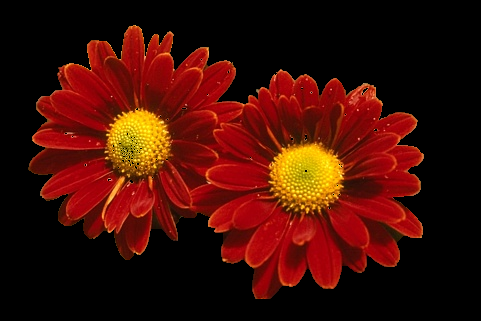
\includegraphics[width=0.3\textwidth]{segmentation}} 
  \caption{Segmentation result}
  \label{fig: } %% label for entire figure 
\end{figure}


\subsection{Step 5: Evaluate segmentation result}

\begin{description}
\item[Input] Segmentation result ($m \times n \times 3$ matrix) and groundtruth ($m \times n$ matrix) from dataset.
\item[Output] A figure that indicates evaluation results (The horizontal axis represents the parameter, the vertical
axis represents the evaluation results.).
\item[Implement] Adjust {\color{blue} threshold} to obtain different segmentation results and draw a bar graph to evaluate grab cut.
\item[Hint] 
\begin{itemize}
\item You can draw PRF (Precision Recall F-measure) bar graph to evaluate.
\item The evaluation is shown is Figure~\ref{fig: evaluation}.
\item A matlab code for computing PRF (Precision Recall F-measure) can be downloaded from website\footnote{\url{http://vision.ouc.edu.cn/~zhenghaiyong/courses/cv/2015spring/assignments/GrabcutCode.zip}}.
\end{itemize}
\end{description}
\begin{figure}[!ht]
  \center{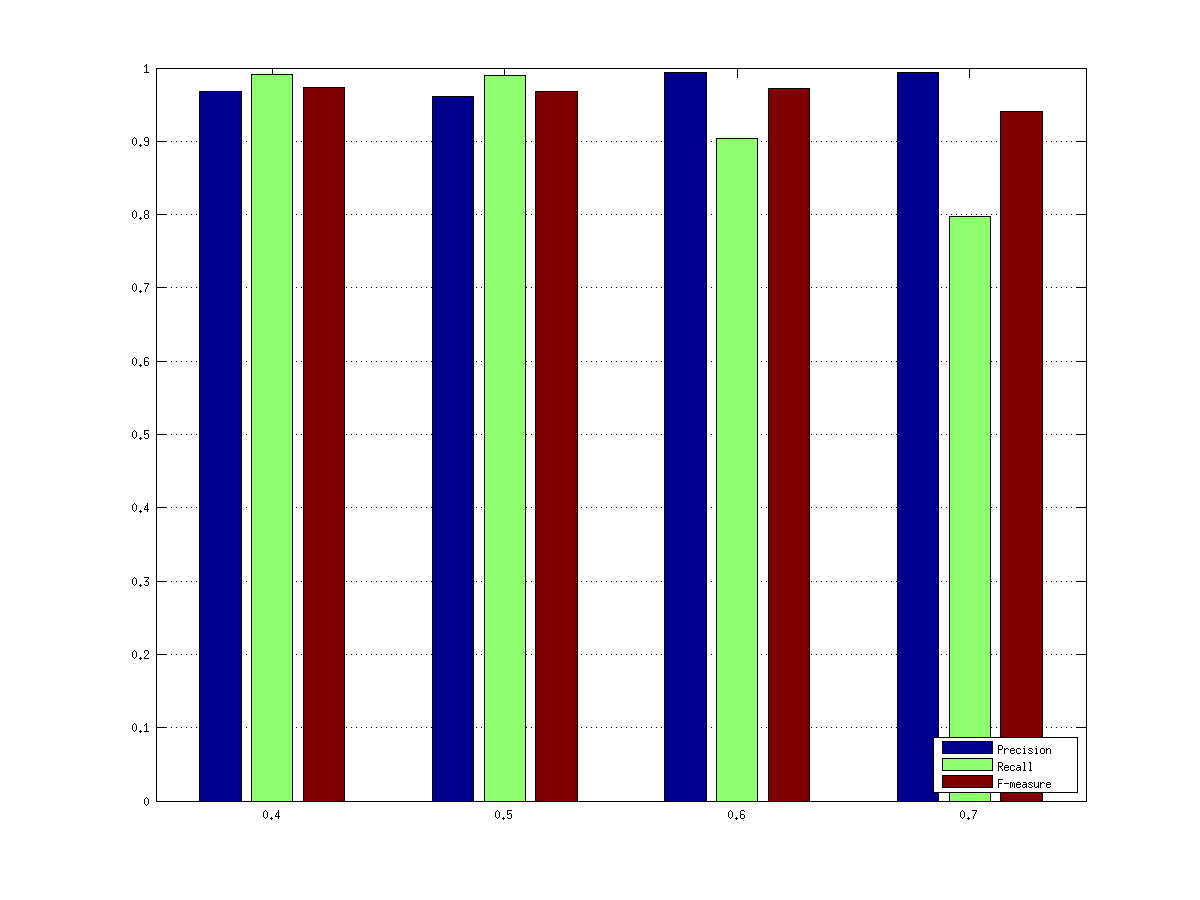
\includegraphics[width=0.3\textwidth]{evaluation}} 
  \caption{PRF bar graph}
  \label{fig: evaluation} %% label for entire figure 
\end{figure}

\subsection{Notes\label{note}}

\begin{itemize}
\item You need to compute the mean value of evaluation result from all images when evaluating.
\item The parameters you choose to adjust can be the followings (adjust at least two parameters for this assignment):
	\begin{itemize}
        \item {\color{blue} threshold} in step 3.
 	\item {\color{blue} size of rectangle} in step 3. 
	\item {\color{blue} times of iteration} in step 5.
	\end{itemize}
\end{itemize}


%\item[Theory] The formulation for histogram distance is as follows:
%\begin{align}
%\chi^2(\textbf{h}_1, \textbf{h}_2) = \sum_{i=1}^{b}\frac{2(h_{1i}-h_{2i})^2}{h_{1i}+h_{2i}}
%\end{align}
%where $\textbf{h}_1$ and $\textbf{h}_2$ ardownloade color histograms of two distinct regions,  $h_{1i}$ and $h_{2i}$ are the $i$th component of $\textbf{h}_1$ and $\textbf{h}_2$ respectively, $b$ is the number of histogram bins. Moreover, both histograms are normalized, i.e. their entries sum up to one.
\section{Mean shift (40 points)}
The whole framework of the implementation for evaluation of mean shift is shown in Figure~\ref{fig:mean}, it may serve as a reference for your assignment. In this part, what you need to do:
\begin{enumerate}
\item Input all images by batch processing (10 points).
\item Adjust two parameters of mean shift (see \ref{step:2}) to get different segmentation results (10 points).
\item Evaluate these segmentation results via two evaluation methods (see \ref{step:3}) (20 points).
\end{enumerate}
Next, I will introduce the implementation and requirement of each step of the framework.
%For this assignment, you will implement different segmentation results by changing the parameters of mean shift. Then, evaluate the different segmentation results by comparing to ground truths.
\begin{figure}[!ht]
\centering
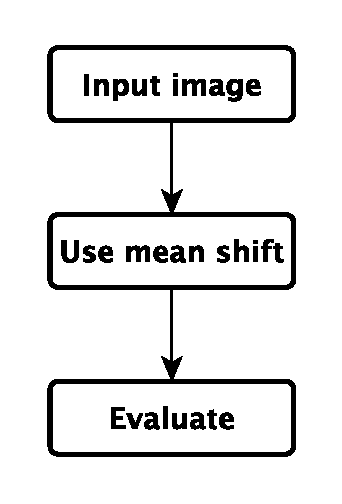
\includegraphics[width=0.2\textwidth]{chartMean.eps}
\caption{Framework of the implementation for evaluation of mean shift.}
\label{fig:mean}
\end{figure}


\subsection{Step 1: Input image}

A simple dataset (BSDS500) can be downloaded from the website\footnote{\url{http://www.eecs.berkeley.edu/Research/Projects/CS/vision/grouping/segbench/}}. The dataset contains input images and groundtruth. Use all images from the dataset for segmentation.
%I just pick one image for segmentation and evaluation as an example. You need to implement 100 images with adjusting at least two parameters.

\subsection{Step 2: Segment via mean shift}\label{step:2}
In this step, you need to adjust the parameters of mean shift to get different segmentation results.
\begin{description}
\item[Input] The color image ($m \times n \times 3~matrix$).
\item[Output] The segmentation results ($m \times n \times 3~matrix$) and label matrixes ($m \times n~matrix$) of different parameters.
\item[Implementation] The parameters of mean shift, which can be adjusted, include:
\begin{itemize}
\item Spatial radius
\item Color radius
\item The number of iterations
\item Iteration accuracy
\end{itemize}
You should adjust at least two parameters to get different segmentation results.
\item[Hint] You can download the source code from the website\footnote{\url{http://www.mathworks.com/matlabcentral/fileexchange/40990-mean-shift-pixel-cluster/content/meanShiftPixCluster.m}}.
\end{description}
\begin{figure}[!ht]
  \centering 
  \subfigure[]{ 
    \label{fig: } %% label for first subfigure 
    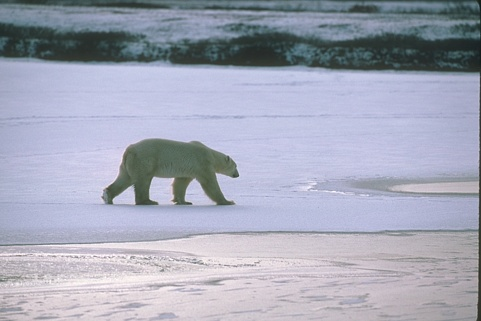
\includegraphics[width=0.3\textwidth]{100007}} 
  \subfigure[]{ 
    \label{fig: result1: b} %% label for second subfigure 
    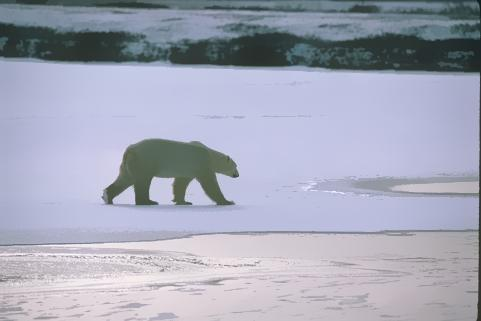
\includegraphics[width=0.3\textwidth]{100007MS}} 
  \caption{The original image and segmentation result.}
  \label{fig: } %% label for entire figure 
\end{figure}

\subsection{Step 3: Evaluate segmentation result with groundtruth}\label{step:3}

In this step, you need to evaluate the different segmentation results from step 2.
\begin{description}
\item[Input] The label matrixes ($m \times n~matrix$) from step 2, the groundtruth matrixes ($m \times n~matrix$) from dataset.
\item[Output] Line chart of the evaluation results. (The horizontal axis represents parameters. The vertical axis represents the evaluation results.)
\item[Implementation] The evaluation methods include: 
    \begin{itemize}
        \item Probabilistic Rand Index (PRI)
        \item Variation of Information (VOI)
        \item Global Consistency Error (GCE)
        \item Boundary Displacement Error (BDE)
    \end{itemize}
You can choose at least two evaluation methods from them.
%For example, Figure~\ref{fig:eval} shows four kinds of evaluation results by adjusting a parameter (spatial radius).


\item[Hint] You can download the source code from the website\footnote{\url{http://www.eecs.berkeley.edu/~yang/software/lossy_segmentation/SegmentationBenchmark.zip}}.

Example: Figure~\ref{fig:eval} shows four kinds of evaluation results (BDE PRI VOI GCE) by adjusting a parameter (spatial radius).

{\color{blue}PS}: The final evaluation result of the dataset is the mean of all images.
\end{description}
    \begin{figure}
      \centering
      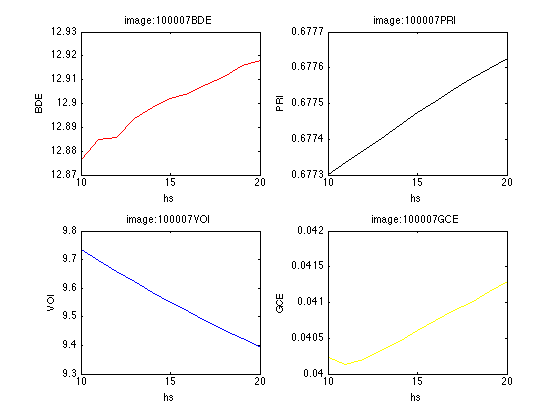
\includegraphics[width=0.45\linewidth]{eval.png} 
      \caption{Line chart of BDE PRI VOI GCE}
      \label{fig:eval} %% label for entire figure 
    \end{figure}

\section{Submission instructions}

\subsection{What to hand in?}

\begin{itemize}
\item Your code (Show your medial result in your code)
\item A report containing the following:
\begin{itemize}
\item Your name at the top
\item A brief explanation of your implementation strategy (in English)
\end{itemize}
\end{itemize}

\subsection{Where to hand in?}

Submit to Piazza in form of a followup below my assignment note.





%\bibliographystyle{plain}
%
%\bibliography{Assignment1} 

%%---------------------------------------------------------------------
\end{document}
